\section{Identifying Posture}

The Biggest hurdle, was and still is identifying and correctly analysing the data. I have had several different aproaches on how to interpret and visualize the data. During my first attempt (Attemt A) i tried to visualized the data in two ways, with Python and Power BI.

Firstly I transformed the data into a CSV which is a commonly used format viable for many different applications

According to the datasheet of the MPU6050 the collected data is "g-force". The accelometer measure in mg and the gyroscope in º/s. 

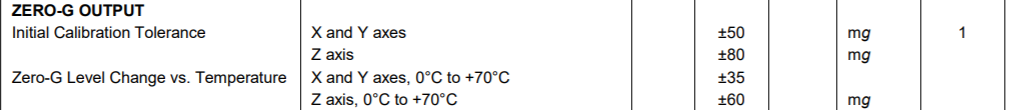
\includegraphics[width=\linewidth]{images/MPU6050_DATA.png}
The entire documentation can be found online \cite{MPU6000D59:online}.

\subsection{Visualising with Python}

I tried to visualize the data using python since it was recommended on a few forums and seamed to be feasible for this task. It actually did work quite well and I have achieved within 2 Days with Python. I have never worked with python before and was happy that I managed to use and apply it within days. 

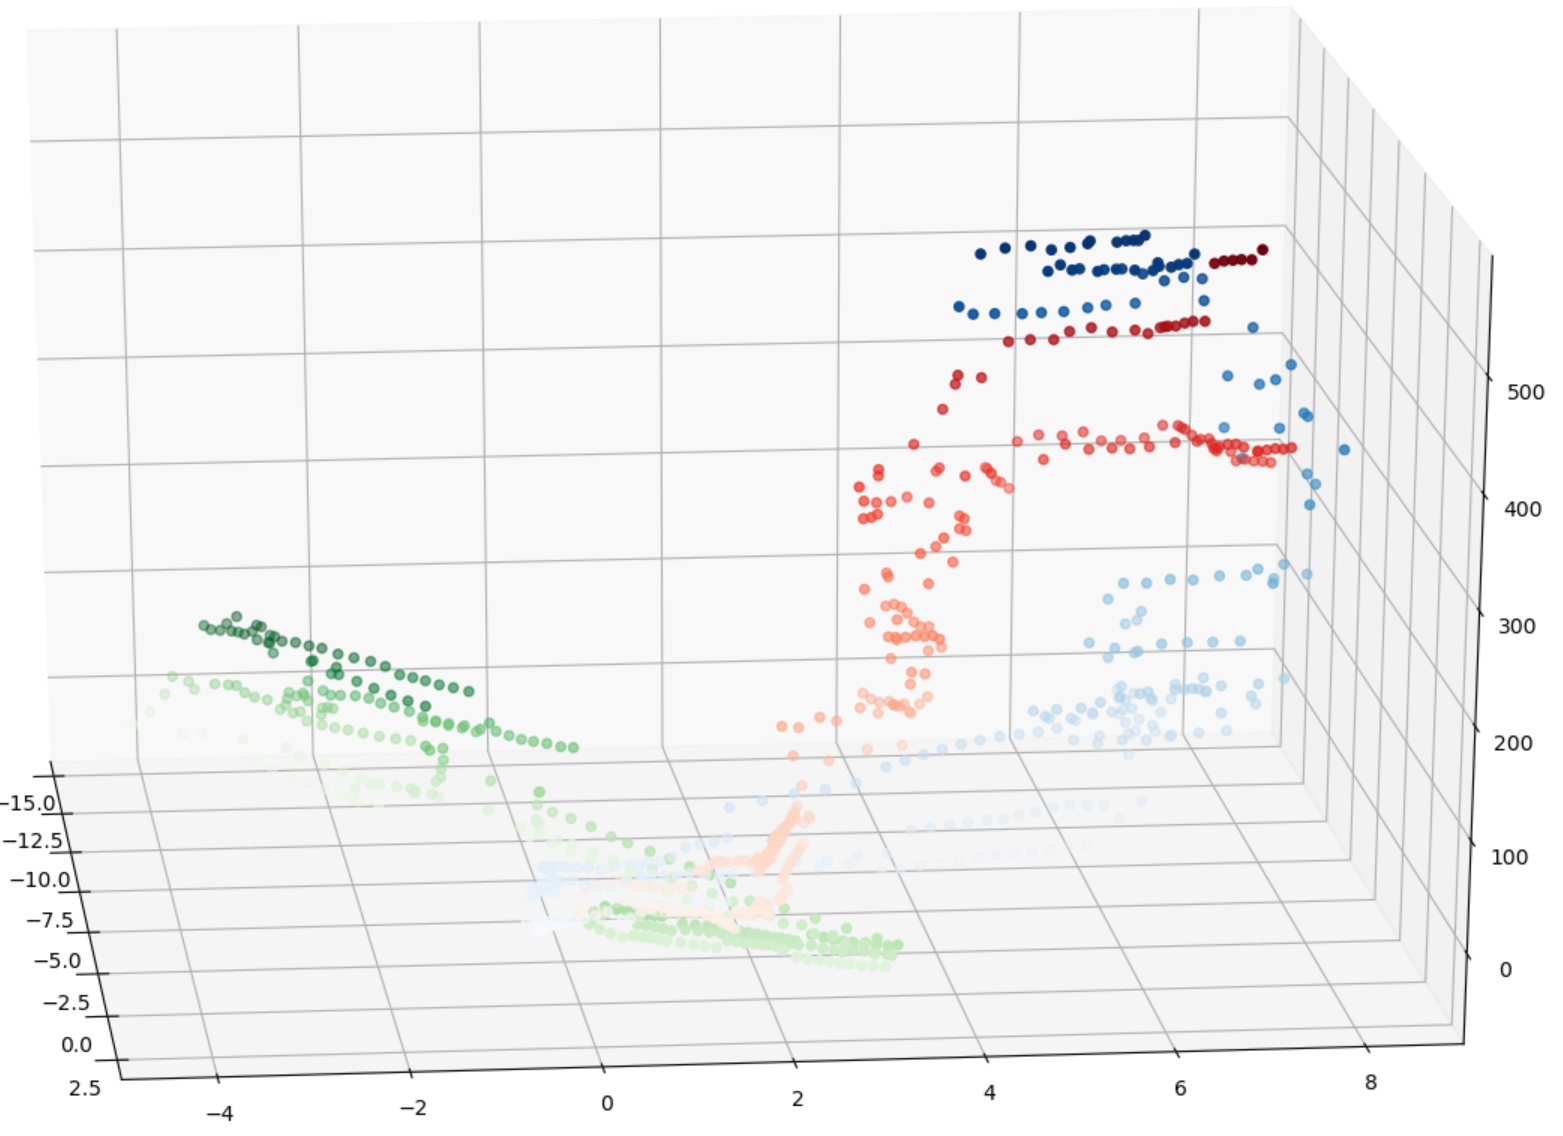
\includegraphics[width=\linewidth]{images/PyVisualisation.png}

Visualised you see my first attempt in showing movement of 3 sensors with the data of the accelometers. The sensors were attached to my shirt with scotch. This is not a perfect solution, which is visible in the different orientation of the green dots. 

Here I tried to add up the movement from the accelometers to see how this stacks up. The Data was not very helpful and i tried to anime the accelometer data directly to see how it changes, this was a bit clearer but still very hard to interpret since it was static data. 

To Visualize I used numpy and matplotlib which are quite handy but still took some time the get used to.
The data was simple display on a grapth (ax) from np arrays:

\begin{lstlisting}
ax.scatter3D(XSXAcc[:,0],XSXAcc[:,1],XSXAcc[:,2], c=XSXAcc[:,2], cmap='Reds')
ax.scatter3D(XSYAcc[:,0],XSYAcc[:,1],XSYAcc[:,2], c=XSYAcc[:,2], cmap='Blues')
ax.scatter3D(XSZAcc[:,0],XSZAcc[:,1],XSZAcc[:,2], c=XSZAcc[:,2], cmap='Greens')
\end{lstlisting}

\subsection{Visualising with Power BI}

Power BI is a very powerfull tool which I was already used to, since we used it at work to visualize project data and quality gates. Therefore it was much easier for me to visualise the data.

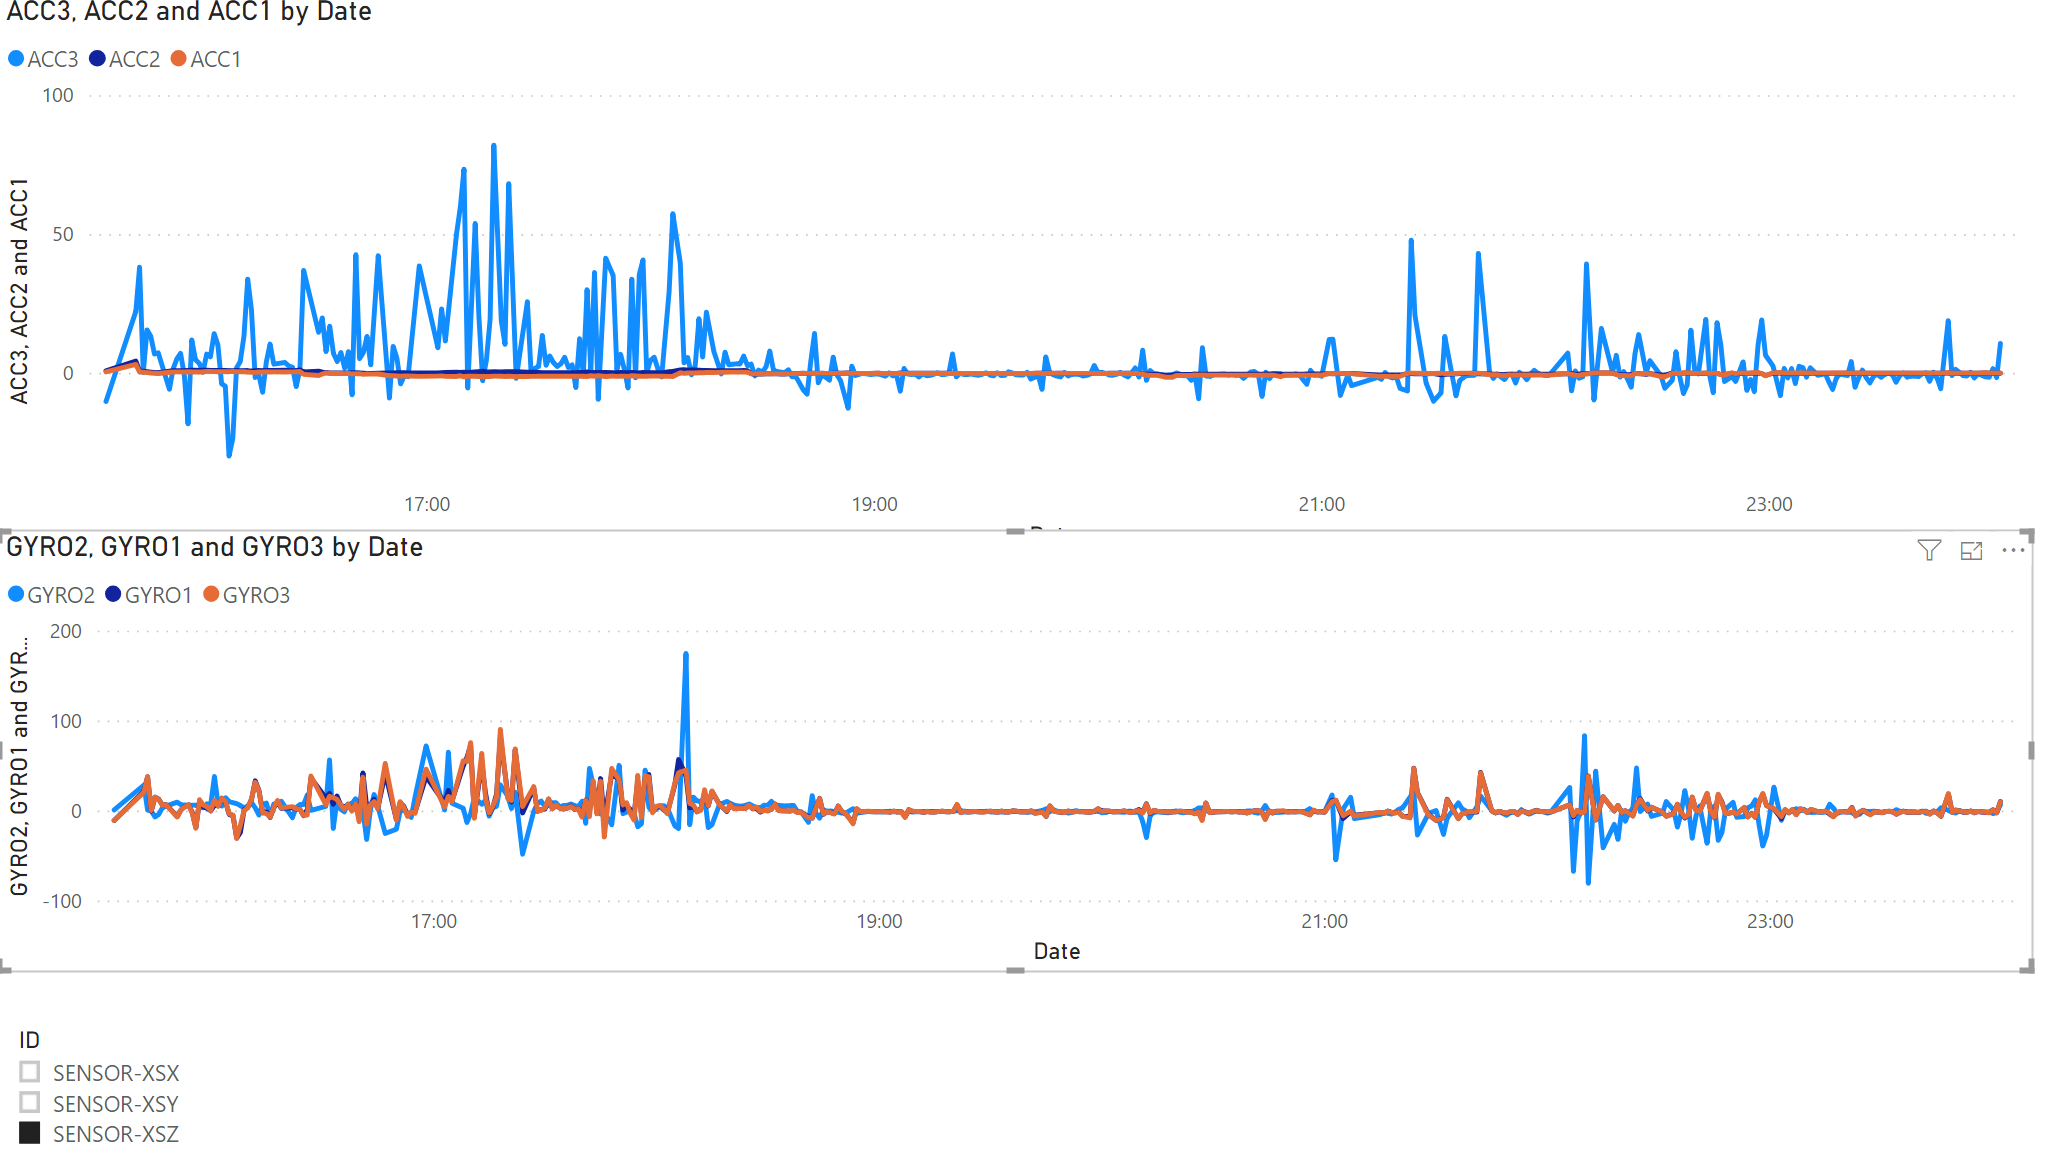
\includegraphics[width=\linewidth]{images/PowerBIVisualisiation.png}

During different attempts of visualising the data i realised, it made sense to visualise it with a 2d graph, since the three dimensional visualisation did not offer any real benefits. Furthermore during this visualisation I also quickly saw, that the data collected had to be incorrect, since the accelometer should never fluctuate as much as id did. The Error was in my code and was quickly fixed, however I still had issues making conclusions for this static data.

\subsection{Real Life Data Visualisation}

The visualisation of static data has a lot of issues, especially when the data is dynamic. Since the collected data would have needed to be compared to a video to really understandt what was going on and what movement hat what effect. Therefore i decided to implement a small webservice which will visualise the data in real time. 

This was achieved with a simple C# MVC website which simply subscribes to the MQTT broker. Here the switch to MQTT and the extra effort for this switch, was highly beneficial.

The Website started small and was simply used to visualize the collected data:

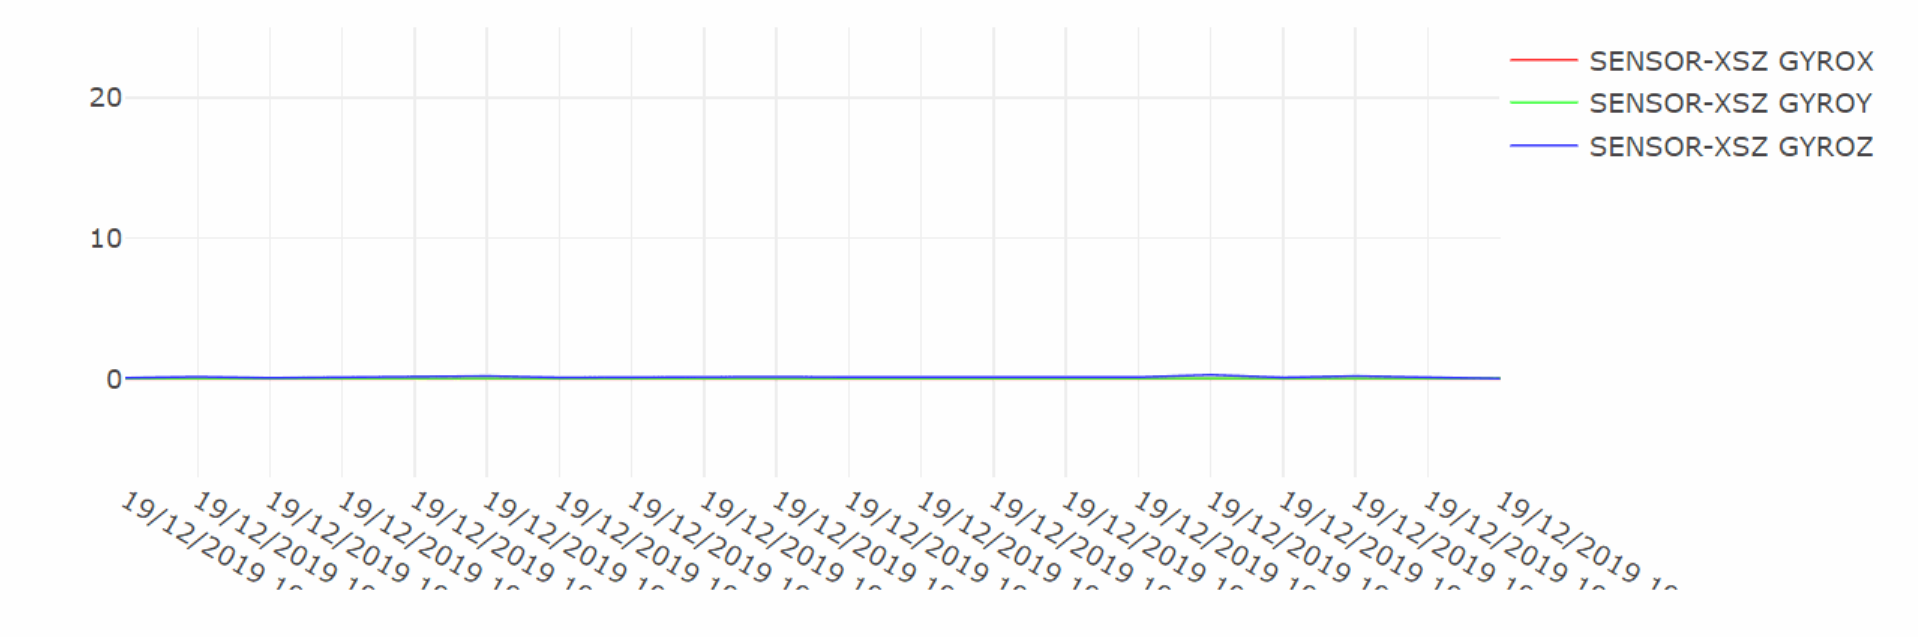
\includegraphics[width=\linewidth]{images/WebVisualisation_SIMPLE.png}

Thanks to this visualisation I was quickly able to understand the data and add additional visualisations and make first conclusions which data was necessary for an analysation.
The Information about the pitch, roll and yaw, was quite simple and only needs the accelometer data.

\begin{lstlisting}
function getRoll(x, y, z) {
    pitch = 180 * Math.atan(x / Math.sqrt(y * y + z * z)) / Math.PI * 4;
    roll = 180 * Math.atan(y / Math.sqrt(x * x + z * z)) / Math.PI * 4;
    yaw = 180 * Math.atan(z / Math.sqrt(x * x + z * z)) / Math.PI * 4;
    return {
        "roll": roll,
        "pitch": pitch,
        "yaw": yaw
    }
}
\end{lstlisting}

With these formula the position of the sensor was really simple to read and visualise. However it was clear that one sensor would not be enough, since its position does not offer enough information about the posture: 

\begin{wrapfigure}[16]{l}{0.3\textwidth}
  \begin{center}
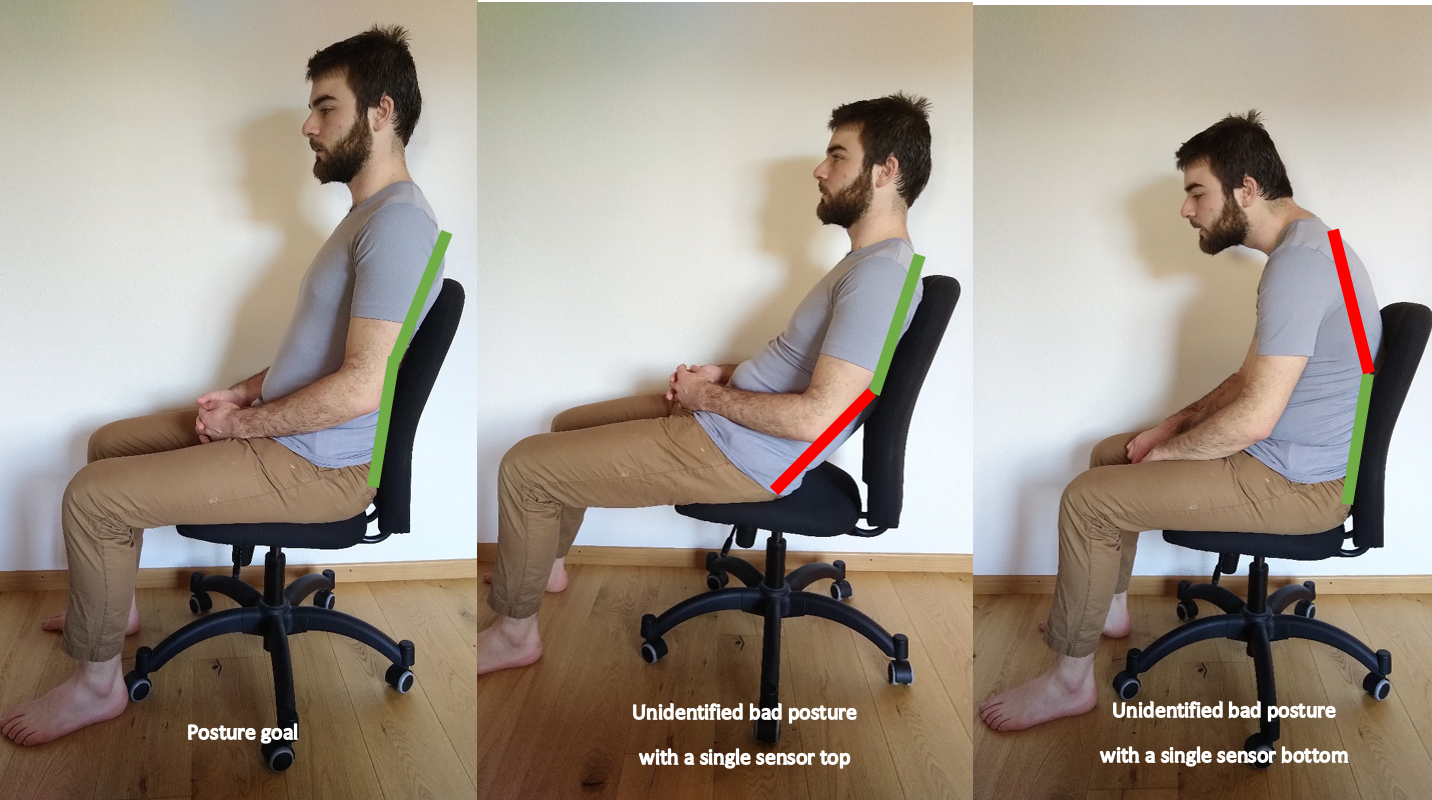
\includegraphics[width=0.3\textwidth]{images/Backposition.png}
  \end{center}
  \caption{Back position}
  \label{fig:BackPos}
\end{wrapfigure}

Therefore a minimum of two sensor would definitely be need to make conclusions from the data. Therefore the website was extended so it can visualise the data of three sensors.